\attrib{David Preston}
%
\begin{quote}
5PH1NX: 5tudent Peer Heuristic for 1Nformation Xchange - we think of it
as a ``curiously trans-media'' use case in peeragogical assessment.
\end{quote}

Over the last several decades technology has driven massive shifts in
the way we communicate and collaborate. Information technology,
socioeconomic trends, an increasingly complex and uncertain future, and
school's failed brand are contributing factors in an emerging discourse
that seeks to align learning with our rapidly changing culture.

Open Source Learning and Peeragogy, two emerging theoretical frameworks
in this discourse, leverage end-to-end user principles of communication
technology to facilitate peers learning together and teaching each
other. In both traditional and liminal learning communities, one of the
major points of contact between education and societal culture is the
purposeful use of assessment. The processes of giving, receiving, and
applying constructive critique makes learners better thinkers,
innovators, motivators, collaborators, coworkers, friends, relatives,
spouses, teammates, and neighbors. Implementing peer-based assessment
can be problematic in schooling institutions where evaluative authority
is traditionally conflated with hierarchical authority, and where
economic and political influences have focused attention on summative,
quantitative, standardized measurement of learning and intelligence.

This is the story of how one learning community is adopting Open Source
Learning and Peeragogical principles to decentralize and enrich the
assessment process.

\begin{quote}
\textbf{Aldous Huxley}: ``Knowledge is acquired when we succeed in
fitting a new experience into the system of concepts based upon our
old experiences. Understanding comes when we liberate ourselves from
the old and so make possible a direct, unmediated contact with the
new, the mystery, moment by moment, of our existence.''
\end{quote}


\subsection{Enter 5PH1NX}

On Monday, April 2, 2011, students in three English classes at a
California public high school discovered anomalies in the day's entry on
their course blog. (Reminder: not so long ago this sentence would have
been rightly interpreted as being science fiction.) The date was wrong
and the journal topic was this:

\begin{quote}
In The Principles of Psychology (1890), William James wrote, ``The
faculty of voluntarily bringing back a wandering attention, over and
over again, is the very root of judgment, character and will. No one is
\emph{compos sui} if he have it not. An education which should improve
this faculty would be the education par excellence.'' How have your
experiences in this course helped you focus your attention? What do you
still need to work on? What elements of the following text (from Haruki
Murakami's \emph{1Q84}) draw your attention and help you construct
meaning? \\[.5cm] The driver nodded and took the money. ``Would you like a
receipt?'' ``No need. And keep the change.'' ``Thanks very much,'' he
said. ``Be care\textbf{f}ul, it looks windy out there. Don't
sl\textbf{i}p.'' ``I'll be careful,'' Aomame said. ``A\textbf{n}d
also,'' the~\textbf{d}river said, facing~\textbf{t}he mirror, ``please
remember: t\textbf{h}ings are not what they seem.''~ Things are not what
they seem, Aomame repeated mentally. ``What do you mean by that?'' she
asked with knitt\textbf{e}d brows. The driver chose his words carefully:
``It's~\textbf{j}ust that y\textbf{o}u're about to do something out of
the ordinary. Am I right? People do not ordinarily climb down the
emergency stairs of the Metropolitan Expressway in the middle of the
day-- especially women.'' ``I suppose you're right.'' ``Right. And after
you do something like that, the everyday loo\textbf{k}~of things might
seem to chang\textbf{e}~a little. Things may
look~\emph{diffe\textbf{r}ent}~to you than they did before. I've had
that experience myself. But don't let appearance\textbf{s} fool you.
There's always only one reality.''
\end{quote}

\subsection{Find the jokers}

{\centering
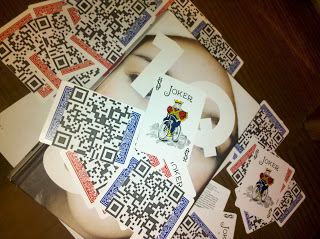
\includegraphics[width=.9\textwidth]{../pictures/jokers.jpg}\par}

\noindent The jokers were real and hidden (without much intent to
conceal) around the classroom and in students' journals. Students
found them and asked questions about the letters in bold; the
questions went unanswered. Some thought it was just another of their
teacher's wild hair ideas. Although they didn't know it yet they were
playing the liminal role that Oedipus originated in mythology. Solving
the riddle would enable them to usher out an old way of thinking and
introduce the new. 

The old way: An authority figure sets the rules,
packages the information for a passive audience, and unilaterally
evaluates each learner's performance. In that context, peeragogical
assessment might be introduced with a theoretical framework, a rubric,
and a lesson plan with input, checks for understanding, and guided
practice as a foundation for independent work.

The new way: In Open
Source Learning the learner pursues a path of inquiry within
communities that function as end-to-end user networks. Each individual
begins her learning with a question and pursues answers through an
interdisciplinary course of study that emphasizes multiple modalities
and the five Fs: mental Fitness, physical Fitness, spiritual Fitness,
civic Fitness, and technological Fitness. Learners collaborate with
mentors and receive feedback from experts, community-based peers, and
the public. They are the heroes of learning journeys. Heroes don't
respond to syllabi. They respond to calls to adventure. Open Source
Learning prepares students for the unforeseen.

By the time they met the 5PH1NX students had learned about habits of
mind, operating schema, digital culture and community,
self-expression, collaboration, free play, autonomy,
confidence/trust/risk, and resilience. These ideas had been reinforced
through nonfiction articles and literary selections such as
Montaigne's Essays, Plato's Allegory of the Cave, Shakespeare's
Hamlet, Sartre's No Exit and others. The first poem assigned in the
course was
Bukowski's~``\href{http://www.youtube.com/watch?v=bHOHi5ueo0A}{Laughing
  Heart}''. \emph{The Gods will offer you chances. Know them. Take
  them.} 

So it is with knowledge and understanding. Today we are presented with
an overwhelming, unprecedented quantity and variety of data in our
physical and virtual lives; to cope we must improve the ways we seek,
select, curate, analyze, evaluate, and act on information.

On the back of each Joker card was a QR code that linked
to a blog page with riddles and clues to a search. At this point
students realized they were playing a game. A tab on the blog page
labeled ``The Law'' laid out the rules of engagement:

\subsection{This is The Law}

\begin{enumerate}
\itemsep1pt\parskip0pt\parsep0pt
\item
  You cannot ``obey'' or ``break'' The Law. You can only make good
  decisions or bad decisions.
\item
  Good decisions lead to positive outcomes.
\item
  Bad decisions lead to suffering.
\item
  Success requires humanity.
\item
  ``For the strength of the Pack is the Wolf, and the strength of the
  Wolf is the Pack.'' -Rudyard Kipling
\item
  ``The Way of the sage is to act but not to compete.'' -Lao Tzu
\item
  Be honorable.
\item
  Have fun.
\item
  Question.
\item
  \emph{Sapere aude}.
\end{enumerate}

This is The Law. After a second set of on-campus and blog quests,
students noticed a shift in 5PH1NX. A couple of weeks before the first
clue was published, during a Socratic seminar on Derrida's concept of
Free Play, a student said, ``We learn best when adults take away the
crutches and there is no safety net.''? The quote was used in the next
clue; students began to realize that the game was not pre-determined.
5PH1NX was evolving in response to their contributions. This is a
manifestation of the hackneyed writing cliché: show, don't tell. The
student's comment was a call to action. The Feats of Wisdom were
designed to engage learners over a vacation break in fun, collaborative,
social media-friendly missions that required engagement in the
community, expansion of their personal learning networks, and
documentation on their blogs. For example:

\paragraph{FEAT \#1.} \emph{Buy a ticket to ``The Hunger Games'' (or any other movie that's
likely to draw a large, young, rowdy audience). Before the lights dim
and the trailers begin, walk to the screen, turn to the audience, and in
a loud, clear voice, recite the ``To be, or not to be\ldots{}''
soliloquy from Hamlet (don't worry if you make a couple mistakes, just
be sure you make it all the way to, ``Be all my sins
remembered.'').~\href{http://alarhsenglitcomp.blogspot.com/2012/12/feats-of-wisdom-1_15.html}{Capture
the event on video \& post it to your blog.}} 

\medskip

Students had been using the Internet without an Acceptable Use Policy
all year; such policies are one-to-many artifacts of a central
authority and far weaker than community norms. So rather than
introduce ``rules'' 5PH1NX simply provided a reminder of the
client-side responsibility.

\subsection{The Emergence of Peeragogical Assessment}

The third page on the Feats of Wisdom blog was entitled
\emph{Identifying and Rewarding Greatness}, where learners were greeted
with the following paragraph:

\begin{quote}
If you see something that was done with love, that pushed the
boundaries, set the standard, broke the mold, pushed the envelope,
raised the bar, blew the doors off, or rocked in some previously
unspecified way, please bring it to the attention of the tribe by
posting a link to it {[}here{]}.
\end{quote}

No one did. Instead, they started doing something more effective. They
started building. One student hacked the entire game and then created
her own version. Other students began to consider the implications for
identifying and rewarding greatness. They realized that one teacher
couldn't possibly observe how 96 students were working over vacation out
in the community and online to accomplish the Feats of Wisdom. In order
to get credit for their efforts they would have to curate and share
their work-process and product. They also realized that the same logic
applied to learning and coursework in general; after all, even the most
engaged, conscientious teacher only sees a high school or college
student a few hours a week, under relatively artificial conditions. The
learner presumably spends her whole life in the company of her own
brain. Who is the more qualified reporting authority? With these
thoughts in mind students created \emph{Project Infinity}, a
peer-to-peer assessment platform through which students could
independently assign value to the thoughts and activities they deemed
worthy. Because the 2011-12 5PH1NX was a three-week exercise in
gamification, \emph{Project Infinity} quickly evolved to include
collaborative working groups and coursework. This was learner-centered
Peeragogical assessment in action; learners identified a need and an
opportunity, they built a tool for the purpose, they managed it
themselves, and they leveraged it in a meaningful way to support student
achievement in the core curriculum.

\subsection{Project Infinity 2 \& Implications for the Future}

Alumni from the Class of 2012 felt such a strong positive connection to
their experience in Open Source Learning and Peeragogical assessment
that they built a version for the Class of 2013. They created
\emph{Project Infinity 2} with enhanced functionality. They asked the
teacher to embed an associated Twitter feed on the course blog, then
came to classes to speak with current students about their experiences.
Everyone thought the Class of 2013 would stand on the shoulders of
giants and adopt the platform with similar enthusiasm. They were wrong.
Students understood the concept and politely contributed suggestions for
credit, but it quickly became evident that they weren't enthusiastic.
Submissions decreased and finally the \emph{Project Infinity 2} Twitter
feed disappeared from the course blog. Learners' blogs and project work
suggested that they were mastering the core curriculum and meta
concepts, and they appeared generally excited about Open Source Learning
overall. So why weren't they more excited about the idea of assessing
themselves and each other? Because \emph{Project Infinity 2} wasn't
theirs. They didn't get to build it. It was handed to them in the same
way that a syllabus is handed to them. No matter how innovative or
effective it might be, \emph{Project Infinity 2} was just another tool
designed by someone else to get students to do something they weren't
sure they wanted or needed to do in the first place. Timing may also be
a factor. Last year's students didn't meet 5PH1NX until the first week
in April, well into the spring semester. This year's cohort started
everything faster and met 5PH1NX in November.~ In January they
understood the true potential of their situation started to take the
reins. As students realized what was happening with the clues and QR
codes they approached the teacher and last year's alumni with a request:
``Let Us In.'' They don't just want to design learning materials or
creatively demonstrate mastery, they want to chart their own course and
build the vehicles for taking the trip. Alumni and students are becoming
Virtual TAs who will start the formal peer-to-peer advising and grading
process. In the Spring Semester all students will be asked to prepare a
statement of goals and intentions, and they will be informed that the
traditional teacher will be responsible for no more than 30\% of their
grade. The rest will come from a community of peers, experts and members
of the public. On Tuesday of Finals Week, 5PH1NX went from five players
to two hundred. Sophomores and freshman have jumped into the fray and
hacked/solved one of the blog clues before seniors did. Members of the
Open Source Learning cohort have also identified opportunities to enrich
and expand 5PH1NX. A series of conversations about in-person retreats
and the alumni community led to students wanting to create a massively
multiple player learning cohort. Imagine 50,000-100,000 learners
collaborating and sharing information on a quest to pass an exam by
solving a puzzle that leads them to a ``Learning Man Festival''? over
Summer break. When 5PH1NX players return from Winter Break in January
they will transform their roles relative to the game and the course.
Several have already shared ``AHA!'' moments in which they discovered
ways to share ideas and encourage collaboration and peer assessment.
They have identified Virtual Teaching Assistant candidates, who will be
coached by alumni, and they have plans to provide peer-based assessment
for their online work. They are also now actively engaged in taking more
control over the collaboration process itself. On the last day of the
semester, a post-finals throwaway day of 30-minute class sessions that
administrators put on the calendar to collect Average Daily Attendance
money, hardly anyone came to campus. But Open Source Learning students
were all there. They have separated the experience of learning from the
temporal, spatial, and cultural constraints of school. They understand
how democracy works: those who participate make the decisions. No one
knows how this ends, but the outcome of Peeragogical assessment is not a
score; it is learners who demonstrate their thinking progress and
mastery through social production and peer-based critique. This
community's approach to learning and assessment has prepared its members
for a complex and uncertain future by moving them from a world of
probability to a world of possibility. As one student put it in a video
entitled ``We Are Superman,'' ``What we are doing now may seem small,
but we are part of something so much bigger than we think. What does
this prove? It proves everything; it proves that it's possible.''

\subsection{Background}

A world in which work looks like what's described in the PSFK think
tank's
\emph{\href{http://www.slideshare.net/PSFK/psfk-presents-future-of-work-report}{Future
of Work Report 2013}} requires a new learning environment.

The problem is that tools and strategies such as MOOCs, videos, virtual
environments, and games are only as good as the contexts in which they
are used. Even the most adept practitioners quickly discover that
pressing emerging technology and culture into the shape of yesterday's
curricular and instructional models amounts to little more than
Skinner's Box 2.0. So what is to be done? How can we use emerging tools
and culture to deliver such an amazing individual and collaborative
experience that it shatters expectations and helps students forget
they're in school long enough to fall in love with learning again?

Education in the Information Age should enable learners to find,
analyze, evaluate, curate, and act on the best available information.
Pursuing an interdisciplinary path of inquiry in an interest-based
community doesn't just facilitate the acquisition of factual knowledge
(which has a limited half-life). The process brings learners closer to
understanding their own habits of mind and gives them practice and an
identity in the culture they'll be expected to join after they graduate.
This requires new literacies and a curriculum that emphasizes mental
fitness, physical fitness, spiritual fitness, civic fitness, and
technological fitness.

Models of assessment that emphasize self-directed and collaborative
Peeragogical principles enrich the learning experience and accelerate
and amplify deep understanding. Because these approaches are pull-based
and generate tens of thousands of multi- or trans-media data points per
learner, they also generate multi-dimensional portraits of learner
development and provide feedback that goes far beyond strengths and
weaknesses in content retention. The long-term benefit is exponential.
Learners who can intentionally direct their own concentration are
empowered far beyond knowledge acquisition or skill mastery. They become
more effective thinkers and -- because they are invested -- more caring
people. This learning experience is of their own making: it isn't
business, it's personal. The inspiration to recreate the process for
themselves and for others is the wellspring of the lifelong learner.

As Benjamin Disraeli put it, ``In general the most successful man in
life is the man who has the best information.'' It is a widely accepted
truism in business that better data leads to better decisions. We now
have the ability to generate, aggregate, analyze, and evaluate much
richer data sets that can help us learn more about helping each other
learn. Sharing richer data in different ways will have the same game
changing effect in learning that it has in professional sports and
investment banking.

Self-directed, collaborative assessment generates an unprecedented
quantity and variety of data that illuminates aspects of learning,
instruction, and overall systemic efficacy. Even a quick look at readily
available freeware metrics, blog/social media content, and time stamps
can provide valuable insight into an individual's working process and
differentiate learners in a network.

In the larger scheme of things, Peeragogical assessment provides direct
access to and practice in the culture learners will be expected to join
when they complete their course of study. Collaboration, delegation,
facilitating conversations, and other highly valued skills are developed
in plain view, where progress can be critiqued and validated by peers,
experts and the public.

But tall trees don't grow by themselves in the desert. Peeragogical
innovation can be challenging in organizational cultures that prioritize
control and standardization; as Senge \emph{et al}. have observed, the
system doesn't evaluate quality when dealing with the unfamiliar, it
just pushes back. In schools this is so typical that it doesn't merit
comment in traditional media. The world notices when Syria goes dark,
but in school, restricted online access is business as usual.

Cultural constraints can make early adopters in technology-based
Peeragogy seem like Promethean risk-takers.~ Whenever the author gives a
talk or an interview, someone asks if he's in trouble.

Learners are not fooled by the rhetoric of in loco parentis or vision
statements that emphasize ``safe, nurturing learning environments.''
With notable exceptions, today's school leaders do not know as much
about technology as the young people for whom they assume
responsibility. Still, learners understand survival: they are fighting
in unfavorable terrain against an enemy of great power. Innovating is
impossible, and even loudly criticizing school or advocating for change
is a risk. As a result many do just enough to satisfy requirements
without getting involved enough to attract attention. Some have also
internalized the critical voices of authority or the failure of the
formal experience as evidence of their own inability: ``I'm just not
good at math.''

How do we know when we're really good at something? Standardized testing
feedback doesn't help learners improve. Most of us don't have a natural
talent for offering or accepting criticism. And yet, as Wole Soyinka put
it, ``The greatest threat to freedom is the absence of criticism.''
Peeragogical interaction requires refining relational and topical
critique, as well as skills in other ``meta'' literacies, including but
not limited to critical thinking, collaboration, conflict resolution,
decision-making, mindfulness, patience and compassion.

Interpersonal learning skills are undervalued in today's schooling
paradigm. Consequently there is an operational lack of incentive for
teachers and learners to devote time and energy, particularly when it
carries a perceived cost in achievement on tests that determine
financial allocations and job security.~ In recent years there has been
increasing pressure to tie teacher compensation, performance evaluation,
and job status directly to student performance on standardized tests.

Some educators are introducing peer-to-peer network language and even
introducing peer-based assessment. But the contracts, syllabi and
letters to students typically stink of \emph{the old way}. These
one-to-many documents are presented by agents of the institution endowed
with the power to reward or punish. To many students this does not
represent a choice or a real opportunity to hack the learning
experience. They suspect manipulation, and they wait for the other shoe
to drop. Learners also don't like to be told they're free while being
forced to operate within tight constraints. Consider this likely
reaction to a policy that is highly regarded in the field:

\begin{quote}
``Students may choose to reblog their work in a public place or on their
own blogs, but do so at their own risk.''

\emph{(What? Did I read that correctly?)}

``Students may choose to reblog their work in a public place or on their
own blogs, but do so at their own risk.''

\emph{(Risk? What risk? The risk of possibly helping someone understand
something that they didn't before, or get a different opinion than the
one they had before? Someone please help me make sense of this.)}
\end{quote}

To effectively adopt Peeragogical assessment in the schooling context,
the community must construct a new understanding of how the members in a
network relate to one another independent of their roles in the
surrounding social or hierarchical systems. This requires trust, which
in school requires significant suspension of disbelief, which -- and
this is the hard part -- requires actual substantive, structural change
in the learning transaction. This is the defining characteristic of Open
Source Learning: as the network grows, changes composition, and changes
purpose, it also changes the direction and content of the learning
experience. Every network member can introduce new ideas, ask questions,
and contribute resources than refine and redirect the process.

This isn't easy. A member in this network must forget what she knows
about school in order to test the boundaries of learning that shape her
relationship to content, peers, and expert sources of information and
feedback. This is how the cogs in the machine become the liminal heroes
who redesign it. Having rejected the old way, they must now create the
rituals that will come to define the new. They are following in the path
of Oedipus, who took on the inscrutable and intimidating Sphinx, solved
the riddle that had killed others who tried, and ushered out the old
belief systems to pave the way for the Gods of Olympus.~ Imagine what
would have happened if Oedipus had had the Internet.

\refstepcounter{labelstepper}
\label{sphinx-end}
